\documentclass[10pt]{article}

\usepackage[utf8]{inputenc}
\usepackage[spanish]{babel}


\usepackage{dirtytalk}

\usepackage[hidelinks]{hyperref}

\usepackage[a4paper, lmargin=0.14\paperwidth, rmargin=0.14\paperwidth, tmargin=0.1111\paperheight, bmargin=0.1111\paperheight]{geometry}


\usepackage{graphicx}
\graphicspath{ {images/} }


\usepackage{fancyhdr} % Headers and footers
\pagestyle{fancy} % All pages have headers and footers
\fancyhead{} % Blank out the default header
\fancyfoot{} % Blank out the default footer
\fancyhead[C]{ \today \ $\bullet$ PyS $\bullet$ Consumo Energético de los Centros de Computación } % Custom header text
\fancyfoot[RO] {\thepage}



\begin{document}

%----------------------------------------------------------------------------------------
%	TITLE SECTION
%----------------------------------------------------------------------------------------
	\begin{titlepage}
      \centering
          %\includegraphics[width=0.15\textwidth]{example-image-1x1}\par\vspace{1cm}
          {\scshape\LARGE Universidad de Valladolid \par}
          \vspace{1cm}
          {\scshape\Large Profesión y Sociedad.\par}
          \vspace{1.5cm}
          {\huge\bfseries Consumo Energético de los Centros de Computación \par}
          \vspace{2cm}
          {\large
          \textsc{Amigo Alonso, Alberto}\\[2mm] % Your name
          \textsc{Delgado Álvarez, Sergio}\\[2mm] % Your name
          \textsc{García Prado, Sergio}\\[2mm] % Your name
          \textsc{Iglesias Cortijo, David}\\[2mm] % Your name

          \vspace{-5mm}
          }

          \vfill
		% Bottom of the page
		{\large \today\par}
	\end{titlepage}

%----------------------------------------------------------------------------------------
%	TABLE OF CONTENTS
%----------------------------------------------------------------------------------------

	\clearpage
	\tableofcontents

%----------------------------------------------------------------------------------------
%	TEXT
%----------------------------------------------------------------------------------------

	\clearpage
  \section{Introducción}
	\label{sec:introducion}
    \paragraph{}


  \section{Análisis sobre el consumo}
  \label{sec:analisis}
  	\paragraph{}
	Como es bien conocido, el gran problema de los actuales centros de datos y de supercomputación, que viene siendo arrastrado desde el pasado, es la gran cantidad de energía que necesitan para su funcionamiento. Es por ello, que el primer paso en este estudio será analizar de dónde procede esta necesidad energética y cuantificar el consumo medio de un centro de computación.

    \subsection{Dentro de un centro de datos}
			\paragraph{}
            Como se muestra en la Figura \ref{image:datacenter}, un centro de datos consta básicamente de los siguientes elementos estructurales:
                        
            \begin{figure}[htpb!]
				\begin{center}
					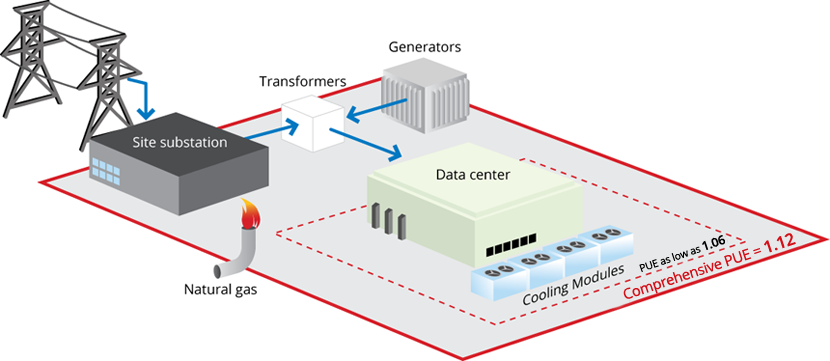
\includegraphics[width=0.75\textwidth]{pue-comprehensive}
					\caption{Esquema de un centro de datos.\cite{google:dc-schema}}
					\label{image:datacenter}
				\end{center}
			\end{figure}
            
            \begin{enumerate}
            	\item \textbf{Proveedores de energía:} Estos son los componentes que alimentan a los servidores de cómputo y al resto de elementos del recinto. Esta alimentación se suele dar en forma de corriente alterna y es necesario un \textbf{transformador} para convertirla en corriente continua usable por las máquinas. La energía puede tener varios orígenes, recomendándose el uso híbrido de ambos:
                	\begin{itemize}
                		\item \textbf{Subestaciones eléctricas} mediante las cuales se puede traer energía del exterior.
                        \item \textbf{Generadores} propios del centro, que serán un recurso mas económico como complemento, pero mas caro en caso de ser la única fuente proveedora. 
                	\end{itemize}
                    
                  \item \textbf{Servidores de datos:} Son los elementos que gestionan la carga útil del centro. Están compuestos por los elementos típicos de una arquitectura Von Neumann: procesador, memoria principal y almacenamiento. Estos son usados con mecanismos de partición de los recursos para crear clusters que puedan ser usados individualmente.
                  
                  \item \textbf{Sistema de refrigeración:} Como será explicado mas adelante, la gran cantidad de calor que liberan los recursos electrónicos convierte en necesario el uso de sistemas que mitiguen dicha energía.
            \end{enumerate}
            
   \newpage
   
   \subsection{Consumo por elemento}
			\paragraph{}
            De los elementos de un centro de datos que se han presentado a un nivel de abstracción elevado, los proveedores de energía son los únicos que no son útiles en el estudio del consumo energético del recinto ya que ellos de por sí no tienen un consumo asociado a su uso.
            
            \paragraph{}
            Los servidores de datos, sin embargo, son los componentes del centro que más energía consumen y merecen por ello un análisis detallado sobre el gasto que acarrean: \cite{datacenters:consumo}
            
            \paragraph{}
            Para ello es fundamental, en primer lugar, la cuantificación de la potencia que utilizan las granjas de servidores de los centros de datos. Como guía, se estima

  \section{Impacto medioambiental}
	\label{sec:impacto}

    \paragraph{}
		Los centros de computación provocan una gran alteración del medio ambiente, ya que requieren mucha energía para poder funcionar y además desprenden grandes cantidades de calor. Por tanto el impacto medioambiental es grande. A continuación se tratarán las formas en las que los centros de computación afectan gravemente al medio ambiente.

    \subsection{Gasto energético}
	  	\paragraph{}
		Los centros de computación siempre han consumido grandes cantidades de energía, al principio este gasto no se tenía demasiado en cuenta pero en los últimos años el consumo energético ha tomado gran importancia, de tal forma que muchas empresas han destinado gran cantidad de recursos a reducir este consumo de una forma u otra. A continuación se podrá observar a qué se destina la energía en un centro de computación. 
        
        \begin{figure}[htpb!]
				\begin{center}
					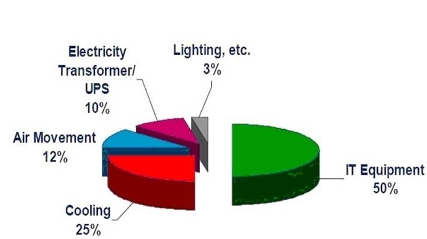
\includegraphics[width=0.75\textwidth]{tech-consumo}
					\caption{Consumo de energía.\cite{technoreeze: impacto}}
					\label{image:tech-consumo.PNG}
				\end{center}
		\end{figure}
            
        \begin{itemize}
        \item Iluminación: El sistema de iluminación consume aproximadamente un 3\% de la energía total del centro, cabe destacar que aproximadamente un cuarto de la energía destinada a iluminación está reservada para la iluminación de emergencia del centro.
        \item Suministro ininterrumpido: Un 10\% de la energía total se reserva para proveer un suministro ininterrumpido de la energía. Esto conlleva que aunque el flujo de energía hacia el resto de sistemas sea constante, hay que preveer una actuación de emergencia en el caso de que el sistema energético principal falle, de tal forma que este sistema de energía ininterrumpido abastecería la energía suficiente a los equipos para evitar que estos pudieran recibir daño alguno
        \item Aire acondicionado: un 12\% de la energía se destina al aire acondicionado, es recomendable que un centro de procesamiento tenga una temperatura comprendida entre los 81 y los 21 grados centígrados, y que la humedad relativa esté comprendida entre el 45\% y el 65\%.
        \item Refrigeración: La refrigeración de los equipos es crucial para su buen funcionamiento, hay que tener en cuenta que estos equipos están funcionando de forma ininterrumpida, por tanto es inevitable su calentamiento. Es muy importante una buena refrigeración y el 25\% de la energía suele destinarse a ella.
        \item Equipamiento: El 50\% restante de la energía se utiliza para abastecer todo el sistema informático y electrónico, para que todos los equipos funcionen correctamente y tengan la energía necesaria para trabajar.
        \end{itemize}
        
	  \subsection{Impacto hidráulico}
	  	\paragraph{}
		El consumo de agua es uno de los grandes problemas de los centros de datos, según investigadores del \textit{Imperial College} de Londres se pueden estar consumiendo hasta unos 200 litros de agua en la descarga de un gigabyte de datos. Son cifras preocupantes ya que en Europa se consumen unos 2GB al mes por persona y en Estados Unidos la cifra asciende a unos 4GB. 
        
        \paragraph{}
        Este cálculo se realiza teniendo en cuenta el consumo hidráulico que precisa un centro de datos para refrigerar correctamente todo su equipamiento, así como la energía necesaria para funcionar. De tal forma que los centros de datos son unos grandes consumidores de agua, problema que ha llevado a las empresas a tratar de proporcionar ciertas soluciones, por ejemplo Microsoft ya tiene prototipos para tratar de construir un centro de computación bajo el mar, de tal forma que obtendría una refrigeración natural aunque tal vez provoque otros problemas en el entorno marino, que se mencionarán más adelante, pero el problema de la refrigeración estaría solucionado.
        
	  \subsection{Emisiones de dióxido carbono}
	  	\paragraph{}
		
        
	  \subsection{Impacto sobre el suelo terrestre}
	  	\paragraph{}

	  \subsection{Fauna y flora del entorno}
	  	\paragraph{}



  \section{Estrategias de optimización}
	\label{sec:estrategias}

  	\paragraph{}
		Como ya se ha visto en la sección \ref{sec:analisis}, los grandes centros de computación producen un elevado consumo energético, lo que repercute negativamente en la productividad de los mismos, y por lo tanto en los beneficios económicos. Además, tal y como vimos en la sección \ref{sec:impacto}, el entorno medioambiental en la zona donde estos se localizan puede verse afectado negativamente.


		\paragraph{}
		Debido a estos factores, las organizaciones encargadas de gestionar este tipo de centros, cada vez más, dedican un alto grado de esfuerzo para tratar de reducir su consumo energético. Existen numerosos documentos emitidos por distintas entidades de prestigio que tratan de proponer un conjunto de estrategías o puntos de revisión en los sistemas para tratar de reducir su consumo energético. Algunos de los más importantes son los ofrecidos por: \emph{EnergyStar}\cite{energy-star:guide}, \emph{Intel}\cite{intel:guide}, \emph{NRDC}\cite{nrdc:guide}, \emph{Energy}\cite{energy:guide}, \emph{Google}\cite{google:case_study}, \emph{Cisco}\cite{cisco:guide} o  \emph{IBM}\cite{ibm:guide} aunque existe una extensa cantidad de información al respecto.

		\paragraph{}
		En esta sección se ha tratado de combinar el conjunto de técnicas recomendadas por los documentos citados anteriormente tratando de conseguir abarcar el mayor número de puntos posibles evitando la repetición de información. A continuación se exponen dichas técnicas según el objetivo para el que van dirigidas:


		\subsection{Virtualización}

			\paragraph{}
			Uno de los puntos en común en todas las guías citadas es su enfasis en la \textbf{virtualización}. Esta técnica se refiere a la capacidad de abstraer la visión de un conjunto de servidores de manera que desde el exterior sean vistos como una única máquina. A pesar del coste computacional destinado a dicho fin, con esto se consiguen reduciones en el consumo energético debido al aumento del uso de las máquinas.

			\paragraph{}
			Típicamente se asignaba un servidor físico por aplicación o sistema, con lo cuál, mientras no se utilizara dicho sistema, el servidor permanecía inactivo consumiendo energía, por lo que la productividad energética de los mismos no era la óptima. Con las estrategias actuales de virtualización se pretende tratar todas las aplicaciones que se ejecutan en el centro de datos como procesos de una única máquina virtualizada. Esto se ilustra gráficamente en la figura \ref{image:virtualization}. Con lo cuál, se consigue que los servidores aprovechen mucho más sus capacidades de cómputo, ya que pueden realizar operaciones relativas a cualquiera de las aplicaciones. Por tanto, la complejidad que gana el centro de datos debido a esta opción es altamente recompensada con la reducción del consumo energético.


			\begin{figure}[htpb!]
				\begin{center}
					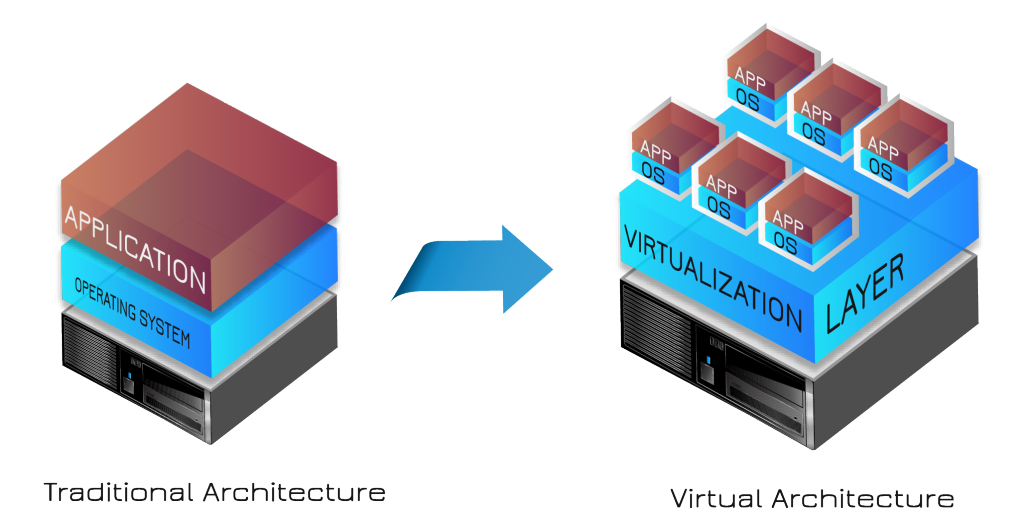
\includegraphics[width=0.75\textwidth]{virtualization}
					\caption{Virtualización de Servidores.\cite{exelos:virtualization}}
					\label{image:virtualization}
				\end{center}
			\end{figure}

		\subsection{Apagado Automático}

			\paragraph{}
			Una de las ventajas del uso de estrategias de virtualización es la capacidad de abstracción que se obtiene. Con esto, se consigue hacer independiente la capa de software de la de hardware. Por tanto, se añade la posibilidad de poder añadir o eliminar servidores físicos al sistema global en tiempo de ejecución, según las necesidades en cada momento. Esta idea se enmarca dentro de un concepto más global denominado \textbf{escalabilidad}:

			\say{La escalabilidad es la propiedad deseable de un sistema, una red o un proceso, que indica su habilidad para reaccionar y adaptarse sin perder calidad, o bien manejar el crecimiento continuo de trabajo de manera fluida, o bien para estar preparado para hacerse más grande sin perder calidad en los servicios ofrecidos}\cite{wikipedia:escalabilidad}.

			\paragraph{}
			Por tanto, una correcta gestión del número de servidores activos en el centro de datos, según las necesidades requeridas en cada momento puede reducir el consumo energético global en gran medida. Para la implementación de la automatización de esta estrategia se utilizan umbrales de utilización del sistema a partir de los cuales encender o apagar las máquinas.


		\subsection{Gestión de temperatura}

			\paragraph{}
			La refrigeración de los grandes centros de datos es un tema que genera mucha controversia, debido a las distintas opiniones acerca de la temperatura óptima que debe tener la sala en la cual se localizan los racks de servidores. Las distintas propuestas se pueden englobar dentro del rango de 15 a 30 grados Celsius. A pesar de ello, algo en lo que si coinciden es en el conjunto de estrategias para lograr dicho fin:

			\subsubsection{Flujos de aire}

	 			\paragraph{}
				La idea principal de estra estrategia es la de crear flujos de ventilación de diferentes temperaturas con el fin de que el aire a temperaturas más bajas sea dirigido hacia los servidores mientras que los flujos con altas temperaturas sean dirigidos hacia los puntos de entrada en del sistema de refrigeración. La estrategia habitual es la de direcciónar las corrientes de aire frío de la parte inferior de la sala hacia la superior, tal y como se ilustra en la figura \ref{image:refrigeration}. Esto es así porque el aire caliente tiene un menor grado de densidad, lo cual hace que su peso sea menor y se localice en la parte superior de la sala. Por tanto, se aprovecha este fenomeno natural para generar un flujo de aire frío desde el inferior hacia la zona superior de la sala que atraviesa los racks de servidores reduciendo la temperatura de los mismos.

				\begin{figure}[htpb!]
					\begin{center}
						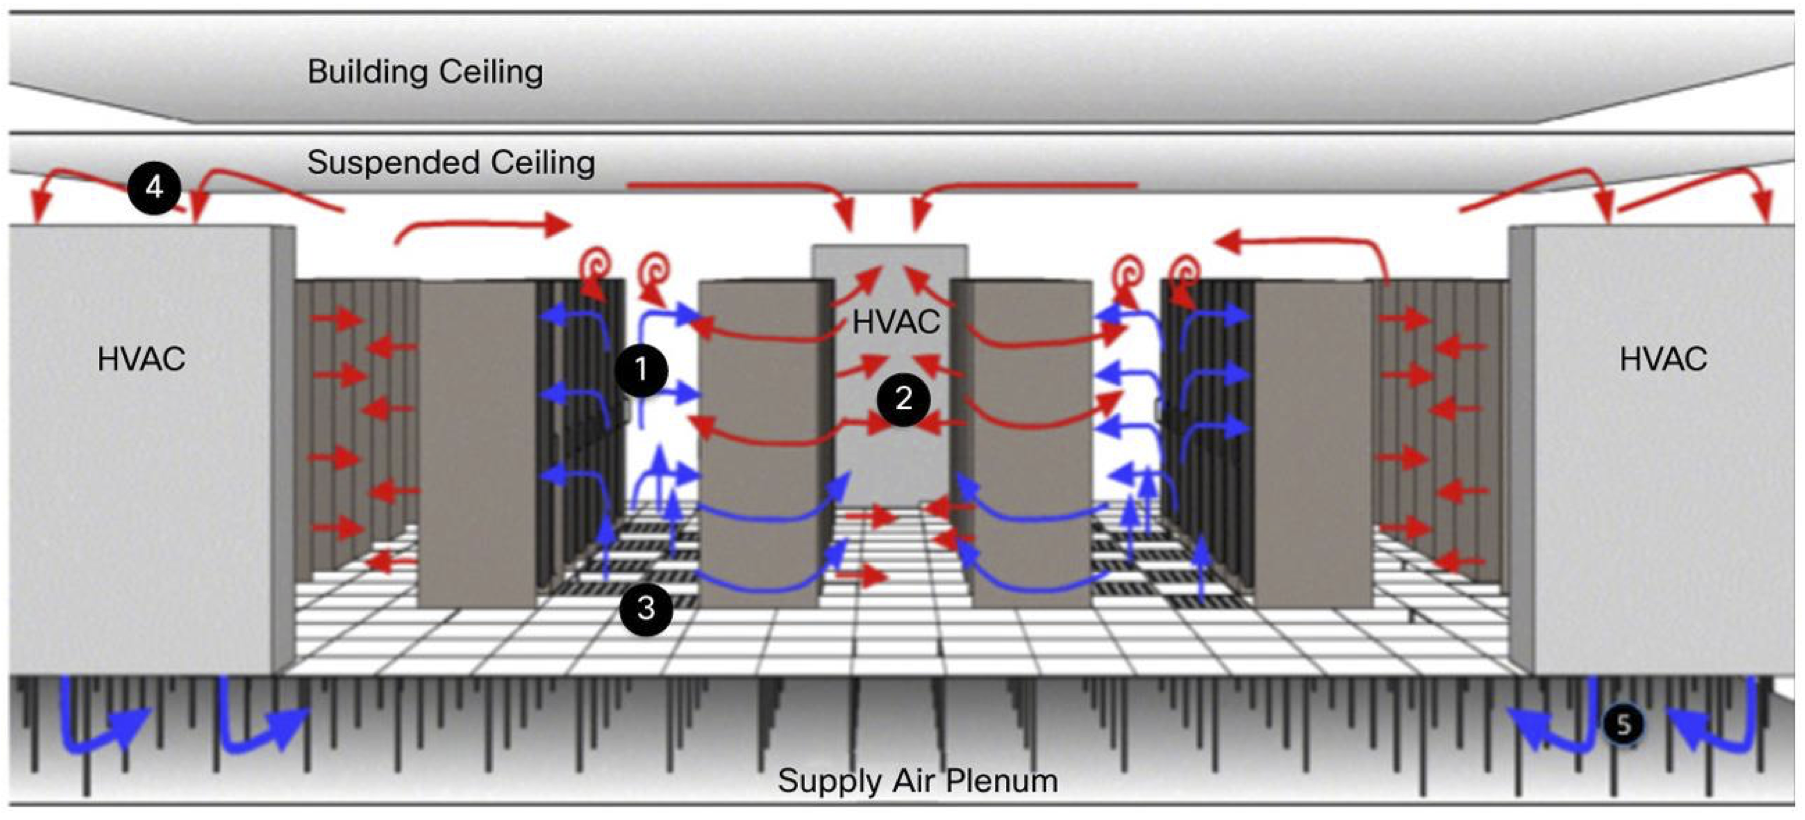
\includegraphics[width=0.75\textwidth]{refrigeration}
						\caption{Refrigeración de Servidores.\cite{cisco:guide}}
						\label{image:refrigeration}
					\end{center}
				\end{figure}

				\paragraph{}
				Una estrategia complementaria a lo citado en el apartado anterior es el control automático de la velocidad de los ventiladores de los racks de servidores, lo cual facilita el aprovechamiento de los flujos de aire según las necesidades de cada zona concreta de la sala.

			\subsubsection{Refrigeración líquida}

				\paragraph{}
				También existen estrategias de refrigeración de servidores mediante circuitos de fluidos a bajas temperaturas en el interior de los racks de servidores. A pesar de ello estas se encuentran en detrimento, debido al riesgo que generan debido a fugas o la dificultad de adaptar la temperatura según zonas específicas

			\subsubsection{Deslocalización hacia zonas frías}

				\paragraph{}
				Otra de las soluciones que se están adoptando para reducir los costes energéticos, en cuanto a la gestión de temperatura, consiste en la deslocalización de los grandes centros de datos hacia zonas cuya condición climática facilite el mantenimiento de temperaturas óptimas. Los destinos escogidos por las organizaciones propietarias son zonas alejadas del ecuador terrestre como zonas de montaña. Tal y como se habló en la sección \ref{sec:impacto}, esto tiene un impacto medioambiental sobre las zonas escogidas pero permite una reducción sobre los costes destinados a la reducción de temperatura de los servidores.

		\subsection{Optimización basada en Inteligencia Artificial}

			\paragraph{}
			Una nueva estrategia de reducción de costes originados por consumo energético en los grandes centros de computación es la optimización mediante inteligencia artificial. Esta es una idea troncal al resto de estrategias vistas anteriormente. El motivo de ello es que se basa en buscar el punto óptimo de gestión de las mismas. En el pasado también se utilizaban técnicas similares para mejorar la productividad pero se caracterizaban por estar basadas en conjuntos de reglas o heurísticas definidas por el ser humano.

			\paragraph{}
			Lo novedoso de las técnicas que cada vez más, se están empezando a utilizar en un amplio rango de disciplinas en que basan la optimización en un concepto denominado \textbf{aprendizaje profundo}, cuya principal idea es la de tratar de aproximarse lo máximo posible a un valor óptimo de una función de coste, a partir de una representación interna del problema en forma de red de \say{neuronas} cuyos valores dirigen la entrada (estado actual del sistema desde el punto de vista del consumo energético) hacia otro valor (conjunto de acciones a realizar como encender o apagar servidores, aumentar la potencia de refrigeración, etc.) idealmente óptimo aprendido previamente.


  \section{Beneficios}
	\label{sec:beneficios}

  	\paragraph{}

  \section{Conclusiones}
	\label{sec:conclusiones}

  	\paragraph{}
%----------------------------------------------------------------------------------------
%	Bibliographic references
%----------------------------------------------------------------------------------------
	\clearpage
  \begin{thebibliography}{9}
  	\bibitem{google:dc-schema}
    	Google: How we do it \url{http://www.google.com/about/datacenters/efficiency/internal/}
        
    \bibitem{datacenters:consumo}
    	Datacenters: Data Center Power Costs and Requirements \url{https://www.datacenters.com/news/infrastructure/135-data-center-power-costs-and-requirements}

    \bibitem{energy-star:guide}
		Enegy Star: 12 Ways to Save Energy in Data Centers and Server Rooms. \newline \url{https://www.energystar.gov/products/low_carbon_it_campaign/12_ways_save_energy_data_center}

    \bibitem{intel:guide}
    Intel: Reducing Data Center Energy Consumption. \newline
 		\url{https://www.irif.fr/~yunes/divers/papers/green/CERN_r04.pdf}

    \bibitem{google:ia}
    Google Blog: Better data centers through machine learning. \newline
		\url{https://googleblog.blogspot.com.es/2014/05/better-data-centers-through-machine.html}

    \bibitem{nrdc:guide}
    NRDC: Data Center Eficiency Assessment. \newline
 		\url{https://www.nrdc.org/sites/default/files/data-center-efficiency-assessment-IP.pdf}

		\bibitem{buildings:guide}
    Buildings: 10 Ways to Save Energy in Your Data Center. \newline \url{http://www.buildings.com/article-details/articleid/6000/title/10-ways-to-save-energy-in-your-data-center}

		\bibitem{energy:guide}
		Enegy: Best Practices Guide for Energy-E cient Data Center Design. \newline
		\url{https://energy.gov/sites/prod/files/2013/10/f3/eedatacenterbestpractices.pdf}

		\bibitem{ibm:guide}
		IBM: Creating a green data center to help reduce energy costs and gain a competitive advantage. \newline
		\url{https://www-935.ibm.com/services/multimedia/GTW03020USEN_186553.pdf}

		\bibitem{colocationamerica:save_energy}
		Colocation America: How Data Centers are Saving Energy. \newline
		\url{https://www.colocationamerica.com/blog/how-data-centers-save-energy}

		\bibitem{elastictree:save_energy}
		ElasticTree: Saving Energy in Data Center Networks. \newline
		\url{http://static.usenix.org/event/nsdi10/tech/full_papers/heller.pdf}

		\bibitem{nolimits:pue}
		No Limits Softwre: Data Center Energy Efficiency – Looking Beyond PUE. \newline
		\url{http://www.nolimitssoftware.com/docs/DataCenterEnergyEfficiency_LookingBeyond.pdf}

		\bibitem{wikipedia:environmental_control}
		Wikipedia: Data Center Environmental Control \newline
		\url{https://en.wikipedia.org/wiki/Data_center_environmental_control}

		\bibitem{google:case_study}
		Google: Google’s Green Data Centers: Network POP Case Study.\newline
		\url{http://static.googleusercontent.com/external_content/untrusted_dlcp/www.google.com/en/us/corporate/datacenter/dc-best-practices-google.pdf}

		\bibitem{sciencedirect:case_study}
		ScienceDirect: Data Center Energy and Cost Saving Evaluation \newline
		\url{http://ac.els-cdn.com/S1876610215009467/1-s2.0-S1876610215009467-main.pdf?_tid=d1bd2bb4-cf33-11e6-94e0-00000aab0f01&acdnat=1483173395_ac49c1e563caaf0fe7fd08f0924993f6}

		\bibitem{cisco:guide}
		Cisco: Data Center Power and Cooling \newline
		\url{http://www.cisco.com/c/en/us/solutions/collateral/data-center-virtualization/unified-computing/white_paper_c11-680202.pdf}

		\bibitem{exelos:virtualization}
		Exelos: Virtualization \newline
		\url{http://exelos.com/solutions/virtualization/}

		\bibitem{wikipedia:escalabilidad}
		Wikipedia: Escalabilidad \newline
		\url{https://es.wikipedia.org/wiki/Escalabilidad}

		\bibitem{technoreeze: impacto}
		Technoreeze: Uso energético de un centro de datos \newline
		\url{http://www.technoreeze.com/es/2011/07/01/datacenters-sostenibles-energia-diseno-e-impacto-ambiental/}
        
        \bibitem{inf-tek: dist-eng}
        inf-tek: distribución energética \newline
        \url{http://inf-tek.blogspot.com.es/2010/10/52-aspectos-electricos-del-centro-de.html}
        
        \bibitem{bbc: g-hidraulico}
        bbc: gasto hidráulico \newline
        \url{http://www.bbc.com/mundo/noticias-37506750}
        
        
        
	\end{thebibliography}

\end{document}
